The use of \mrs is a key aspects to obtain effective solutions in several real world
applications such as for example \footnote{See for example the Kiva system used by Amazon in their warehouse https://www.wired.com/2009/01/retailrobots/.}.
\\
More particularly,
this thesis addresses the cooperation of a team of mobile robots in logistic missions.
The main aspects studied herein are strategies for effective logistic performance,
agent's coordination, scalability and applicability in real-life situations.
In our logistic application the robot team execute specific tasks modeled as exogenous events 
that are characterized by a pick-up location and a delivery location each.
\newline
This introductory chapter presents the context of the research in order to clarify
the motivation and significance of the problem. 
In addition, some guidelines about \mrs in general and, more specifically,
agents in logistic missions are herein introduced to lay the groundwork to 
approach the problem in hands. 
Finally, we provide an overview of the thesis content. 

\section{Context and Motivation}
In recent years, robotics has been one of the scientific fields with the most substantial
advances. Among the different areas of robotics, mobile robotics gained in the last decades 
significant attention roboticists (i.e., researchers on robotics)
around the world. In particular, issues such as autonomous navigation, path planning,
self-localization, coordination of robots, cooperative dynamics, mapping, exploration 
and coverage have become popular topics and have exploited the progress
of artificial intelligence, control theory, real-time systems, sensors’ development,
electronics, communication systems and systems integration \cite{parker}.
\newline
Nowadays, we see different types of robots operating in
different environments as on land, underwater, in the air, suspended on wires,
climbing and so on. This evident growth is extremely motivating for the development
 and contribution of new developments by the community.
\newline
% Da sistemare 
Security applications are a fundamental task with unquestionable impact on
society. Combining this fact with the technological evolution observed in the last
decades, it becomes clear that robot assistance can be a valuable resource by
taking advantage of robots’ ability to cary out tedious or dangerous tasks for a very long time.

The principal scope of the \mrs in logistic application is reduce the costs of the production phase 
and increase the productivity that the robots guarantee in these applications.

In particular, Multi-Robot allocator task for logistic applications
has high utility and is considered as a key area where the use of robots can have a 
dramatic impact on productivity in last decade, especially in terms of strategies for coordinating
teams of robots. 
A key point in for effective application of \mrs in logistic application is to coordiante 
actions of the robot platforms \cite{maxsum}.
However, many of the studies in the literature present unrealistic
simplifications, strong limitations or questionable applicability as illustrated \ref{mrs:logistic}.
Therefore, there is an eminent potential to explore in this context.
\newline
Task allocation for logistic applications problem is very challenging
in the context of \mrs, because agents must navigate autonomously,
coordinate their actions and acquire information
about the surrounding enviroment, possibly with communication constraints and 
should be able to achieve good performance 
on the number of robots in the team and the enviroment's dimension.
Clearly, cooperation among robots is one of the most decisive issues in this context,
since robots most efficiently work together in order to improve the performance of the system as a whole.
All of these features lead to an excellent case study in mobile robotics
and conclusions drawn from such studies may support the development of future
approaches not only in the logistic domain but also in \mrs in
general.

\section{Multi-Robot Systems}
During the last two decades, researchers in the field of mobile robotics have begun 
to investigate problems that involve multiple robot rather than using single robot, and 
research in \mrs has witnessed notorious progress an never before.
In many applications, an autonomous mobile robot equipped with different sensors
may adequately complete a given assignment. However, in several situations. it proves
to be more expensive, less efficient and less robust than using a \mrs. 
In some cases, due to the need of combining different tasks and the dynamics of the environment,
it is only viable to achieve the mission with a multiple distributed autonomous robotic system.  
Some characteristics of \mrs include distributed control, autonomy,
communicative agents and greater fault-tolerance.
A single robot may be vulnerable to hostile environments or attackers, for example, in military actions.
In such scenarios, agents would greatly benefit from the assistance of nearby agents during emergencies,
failures or malfunctions.

Logistic applications can significantly benefit from the use of several robots, however  
(as we discussed above) the effective use of \mrs in logistic applications requires a 
significant effort to delevop an effective and efficient coordinated solution.

Most missions are solved much quicker it robots operate in parallel. 
Increasing robustness and reliability of the solution is also feasible in \mrs by 
introducing redundancies in the capabilities across robot team member and graceful 
performance degradation, remaining functional if some of the agents fail.

One of the main difficulties when approaching these systems is to coordinate
many robots to perform a complex, global task in an efficient manner, maximizing
group performance under a wide range of conditions, with the flexibility to take
advantage of the resources available, embrace the requirements and constraints
imposed and resolve issues like action selection, coherence, conflict resolution and
communication. This cannot be done by just increasing the number of robots
assigned to a task.
A coordination mechanism must exist to establish relationships between agents so
that they can accomplish the mission effectively.

\section{Multi-Robot Systems for logistic applications} \label{mrs:logistic}
Logistic apllication an infrastructure with multiple robots is no different than other Multi-Robot
assignments, in the sense that it incorporates all the previously mentioned
characteristics of \mrs. To understand this problem, it is important to first
introduce the definition of logistic application.

\begin{mydef}
    The industrial logistics is the process of planning, organization and control of all the activities of handling and storage of goods, which, starting from the suppliers and reaching up to the end user, guarantee an adequate level of service to the customer consistent with the costs to it associated
    \footnote{See Basic concepts of Industrial Logistics and Logistics System https://elearning.unito.it/sme/pluginfile.php/36284/mod\_folder/content/0/LOGISTICA}.
\end{mydef}

A traditional warehouse employee typically spends most of his or her time walking 
around the warehouse to gather all of the items for an order. In manual warehouse,
a picker might walk between seven and fifteen miles per shift \footnote{http://www.businessinsider.com/working-conditions-at-an-amazon-warehouse-2013-2?IR=T}. 
To save labor by reducing the time spent walking, a lot company adopt \mrs to improving 
the productivity and have an efficient service for customers.

Many real-world applications of \mrs require agents to operate
in known common environments. 
Our logistic scenario is a map of laboratory for industry 4.0 (ICE lab) with a modern production line,
extended with equipment for augmented reality and digital production, and connected with the university
computational platform plus new hubs.

Below is reported the Figure \ref{fig:ICE lab} of the Industrial Computer Engineering Laboratory used in our 
logistc scenario.

\begin{figure} [hbt]
    \centering
    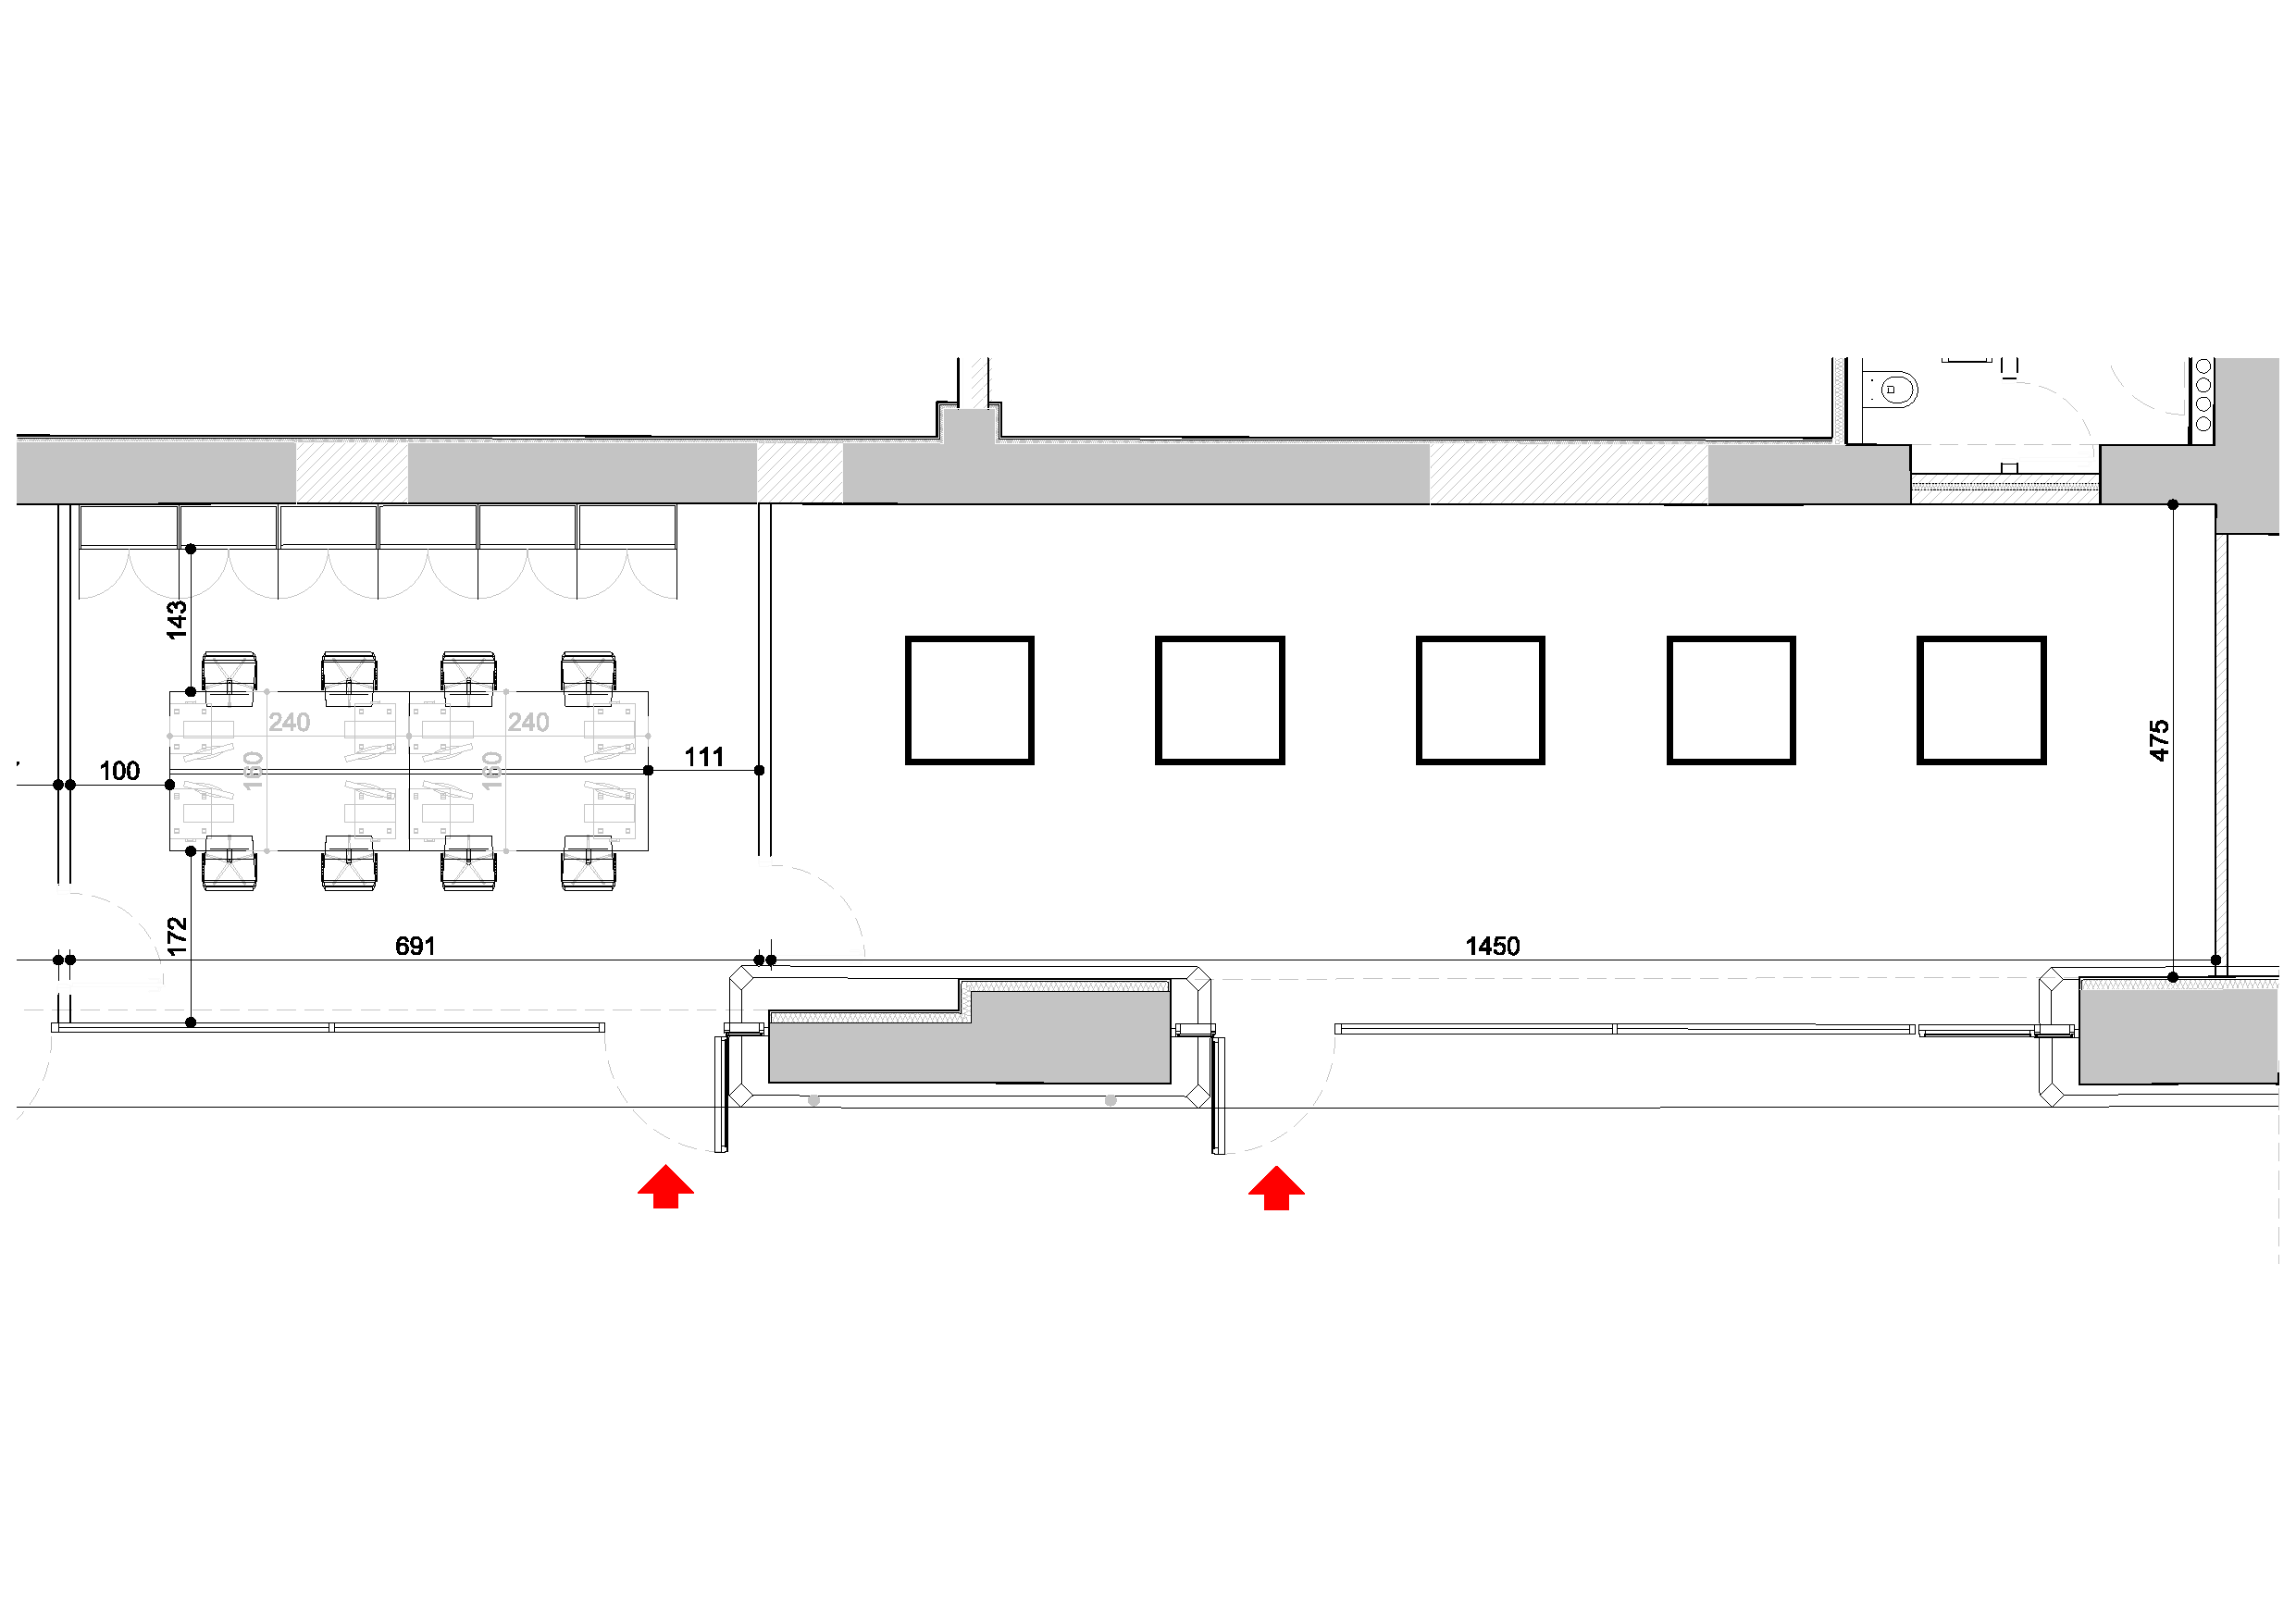
\includegraphics[width=\textwidth]{img/model1.pdf}
    \caption{This is our logistic scenario of Industial Computer Engineering Laboratory}
    \label{fig:ICE lab}
\end{figure}

The map used in the simulator is scaled to have measurements in real enviroment.
In this map we have build the logistic system to perform pick-up and delivery tasks.

An pick-up and delivery task is characterized by a pickup location and a delovery location.
An agent has to move from its current location via the pickup location of the task to
delivery location of the task. When the agent reaches the pickup location, it starts 
to execute the task and the task is removed from the task set.

Wheeled mobile robots mostly operate over a differential drive mechanism. It consists 
of two motors attached wirh wheels on a similar axis. Both motor drives are independent 
of each other's movement. The common access of both motors is known as their center of curvature.
The agent cannot move in the direction along axis. Since both motors can move independently,
their velocities are also different and we can easily vary the trajectory of movement by varying
velocities. The velocities of both drivers must be synchronized in order to move 
the agent in the desired path. 
The robot constructs a two-dimensional geometric representation of its environment
using the laser scanner. It utilizes a combination of this geometric data and odometry
information supplied through the wheel encoders to determine its current location.
For more information about navigation and localization see section \ref{ros:navloc}.
We focus our study to task-allocation problems where one wants to minimize the team 
cost subject to the constraint that each task must be executed by a given number 
of cooperative agents simultaneously.
For \mrs coordination in logistic application there are a lot technique,
in automated warehouse, where agents are constantly engaged with new task, one agent
has to be assigned to each delivery task avoiding collisions with other agents. 
In \cite{mapd} and \cite{mapf} paper has recently received a lot of attention.
They present two decoupled MAPD algorithms, Token Passing (TP) and Token Passing with
Task Swaps (TPTS). Where agents operate in known common enviroments modeled such as 
grids, for each task in a given 2-dimensional 4-neighbor grid with blocked and unblocked 
cells. The multi-agent pathfinding problem is to compute collision-free paths for 
multiple agents, in a post-processing step to adapt its paths to continuous forward 
movements with given traslational velocities and point turns with given rotation velocities.
They take kinematic constraints for instance the robot can turn around only 90 degree at time
and can perform only one task at time. 
In our techniques not consider kinematic constraints and our robots can perform more than one task at time, 
if the capacity of robots are enough.
Then we can allocate more than one task and execute its in one shot.
The agents are constantly engaged with new tasks and have
to navigate between locations where the tasks need to be executed. In particular,
the \mrs for logistic applications, the set of robots must complete a stream attend 
to stream of incoming pickup-and-delivery tasks.
 
\newpage
\section{Thesis contribution}
The contribution of this thesis:
\begin{itemize}
    \item extension of package ROS, implementing an external coordinator for generating tasks and algorithms for composing tasks.
    \item proposing three technique: 
    \begin{enumerate}
        \item baseline greedy approach \srst.
        \item set partition algorithm \sps consider all possible subtask of the task set.
        \item greedy set partition algorithm \gsp proposing an approximation solution with less complexity but efficient subset of task.
    \end{enumerate}
    \item all experiments are executed in a real scenario, precisely on ICE Lab \footnote{See on site the Computer Engineering for Industry 4.0 http://www.di.univr.it/}. 
\end{itemize}

We can see in section \ref{chap:results} that the baseline approach is
the worst algorithm takes more time and takes a more onerous path.
Instead the other two algorithms are quite similar. 
The set partition method is better based on the time and distance traveled but the greedy method,
despite having a lower complexity, obtains excellent results.

The limitation of the set partition approach (\sps) lies in the size of the task set having an exponential complexity
would take too long to compute all possible subset of task.
For this limitation in the experiments we will use a maximum of 9 tasks for this strategy. 

In our approaches we focus on task assignment in base the capacity of the robots for minimize the time traveling and the path distance for every composed task. 

\newpage
\section{Thesis outline}

% da riscrivere

Having answered the questions "What problem is addressed in this thesis?" and 
"Why are we studying this problem?", it id fundamental to answer an additional question,
which is: "How is the problem going to be solved?". This question requires a more 
in-depth answer, that is detailed throughout the rest of thesis.

Initially, an analysis of relevant literature concerning related work to the \mrs 
is conducted in chapter \ref{chap:related}. This allows to formulate the problem 
and extract some weaknesses inherent to previous works.

In chapter \ref{chap:problem} we detail our reference scenario for \mrs coordination and 
well as the formalization of the problem we addressed and the solutions we propose.
Where we introduce the baseline approach for our experiments to then focus on two techniques
which are based on composing task to minimize the task completion time.

Later on, in chapter \ref{chap:ros} a prelimenary framework to solve the \mrs in logistic 
application. 

Finally, the last chapter sums up the work and provides final conclusions and future
directions of research.
% devi completare questo paragrafo aggiungendo:

% -- dire quale problema hai affrontato in particolare: magazzino con mappa realistica, spiega bene il problema di pick up and delivery , descrivere i problemi specifici (path finding, task assignment), citare il avoro su MRS coordination in logistic di koenig e dire che rispetto a quello ci concentriamo sulla capacità dei robot.

% -- descrivere le soluzioni proposte

% -- descrivere il setting sperimentale ed i risultati principali.

% Aggiungere una sezione: Thesis contribution in cui elechi i contributi.

% Aggiungere una sezione thesis outline che riassume i capitoli seguenti.
